%%%%%%%%%%%%%%%%%%%%%%%%%%%%%%%%%%%%%%%%%
% Beamer Presentation
% LaTeX Template
% Version 1.0 (10/11/12)
%
% This template has been downloaded from:
% http://www.LaTeXTemplates.com
%
% License:
% CC BY-NC-SA 3.0 (http://creativecommons.org/licenses/by-nc-sa/3.0/)
%
%%%%%%%%%%%%%%%%%%%%%%%%%%%%%%%%%%%%%%%%%

%----------------------------------------------------------------------------------------
%	PACKAGES AND THEMES
%----------------------------------------------------------------------------------------

\documentclass{beamer}

\mode<presentation> {

% The Beamer class comes with a number of default slide themes
% which change the colors and layouts of slides. Below this is a list
% of all the themes, uncomment each in turn to see what they look like.

%\usetheme{default}
%\usetheme{AnnArbor}
%\usetheme{Antibes}
%\usetheme{Bergen}
%\usetheme{Berkeley}
%\usetheme{Berlin}
%\usetheme{Boadilla}
%\usetheme{CambridgeUS}
%\usetheme{Copenhagen}
%\usetheme{Darmstadt}
%\usetheme{Dresden}
%\usetheme{Frankfurt}
%\usetheme{Goettingen}
%\usetheme{Hannover}
%\usetheme{Ilmenau}
%\usetheme{JuanLesPins}
%\usetheme{Luebeck}
\usetheme{Madrid}
%\usetheme{Malmoe}
%\usetheme{Marburg}
%\usetheme{Montpellier}
%\usetheme{PaloAlto}
%\usetheme{Pittsburgh}
%\usetheme{Rochester}
%\usetheme{Singapore}
%\usetheme{Szeged}
%\usetheme{Warsaw}

% As well as themes, the Beamer class has a number of color themes
% for any slide theme. Uncomment each of these in turn to see how it
% changes the colors of your current slide theme.

%\usecolortheme{albatross}
%\usecolortheme{beaver}
%\usecolortheme{beetle}
%\usecolortheme{crane}
%\usecolortheme{dolphin}
%\usecolortheme{dove}
%\usecolortheme{fly}
%\usecolortheme{lily}
%\usecolortheme{orchid}
%\usecolortheme{rose}
%\usecolortheme{seagull}
%\usecolortheme{seahorse}
%\usecolortheme{whale}
%\usecolortheme{wolverine}

%\setbeamertemplate{footline} % To remove the footer line in all slides uncomment this line
%\setbeamertemplate{footline}[page number] % To replace the footer line in all slides with a simple slide count uncomment this line

%\setbeamertemplate{navigation symbols}{} % To remove the navigation symbols from the bottom of all slides uncomment this line
}

\usepackage{graphicx} % Allows including images
\usepackage{booktabs} % Allows the use of \toprule, \midrule and \bottomrule in tables

%----------------------------------------------------------------------------------------
%	TITLE PAGE
%----------------------------------------------------------------------------------------
\title[Tewogbade Ayobami]{POTENTIAL BENEFIT OF ADOPTING CICD APPROACH FOR THE UDAPEOPLE PROJECT}
\author[Adopting CICD]{Being the Text of a Presentation Prepared\\ by \\~\\ Tewogbade Ayobami}
\institute[]{For Udacity Devops Nanodegree Project 3 submission}
\logo{
\includegraphics[height=1cm]{udapeople.png}}
\date{\today}
%{\today}


\begin{document}

\begin{frame}
\titlepage % Print the title page as the first slide
\end{frame}

\begin{frame}{What is CICD}
	\textbf{CI and CD} are two acronyms frequently used in modern development practices and DevOps.\\
	
	CI/CD is a method to frequently deliver apps to customers by introducing automation into the stages of app development. The main concepts attributed to CI/CD are continuous integration, continuous delivery, and continuous deployment. \\
	
	CI/CD is a solution to the problems integrating new code can cause for development and operations teams (AKA "integration hell"). \\
	
	Specifically, CI/CD introduces ongoing automation and continuous monitoring throughout the lifecycle of apps, from integration and testing phases to delivery and deployment. Taken together, these connected practices are often referred to as a "CI/CD pipeline" and are supported by development and operations teams working together in an agile way with either a DevOps or site reliability engineering (SRE) approach.
	
\end{frame}

\begin{frame}{CICD tools}
\begin{figure}
	\centering
	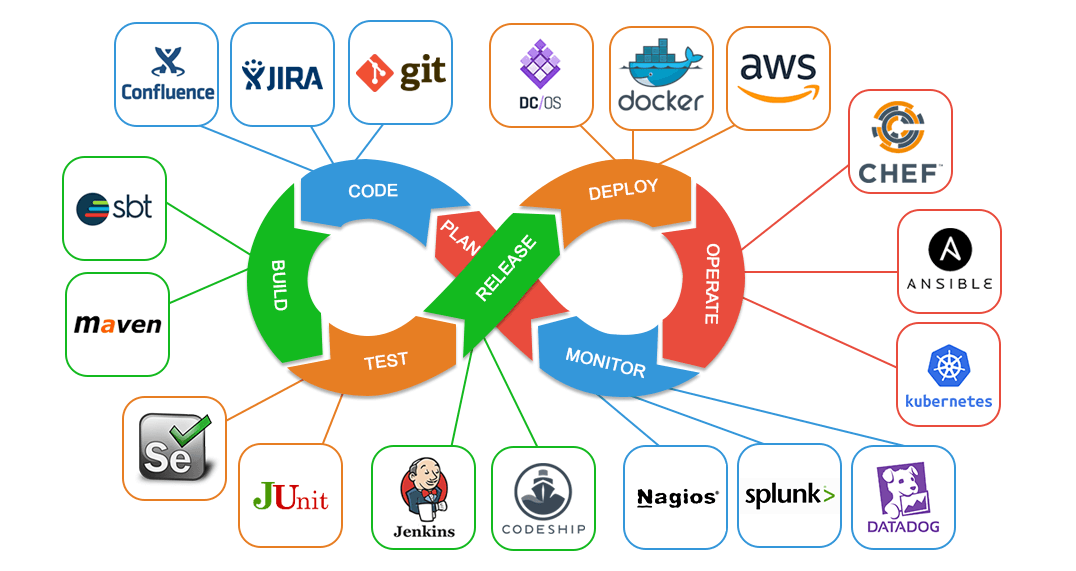
\includegraphics[width=0.9\linewidth]{cicd}
	\caption{}
	\label{fig:cicd}
\end{figure}

\end{frame}

\begin{frame}{Continuous integration}

\begin{block}{What you need (cost)}
	\begin{itemize}
		\item Your team will need to write automated tests for each new feature, improvement, or bug fix.
		\item You need a continuous integration server that can monitor the main repository and run the tests automatically for every new commit pushed.
		\item Developers need to merge their changes as often as possible, at least once a day.
	\end{itemize}
\end{block}
\end{frame}

\begin{frame}{Continuous integration}
	\begin{block}{What you gain}
	\begin{itemize}
		\item Fewer bugs get shipped to production as regressions are captured early by the automated tests.
		\item Building the release is easy as all integration issues have been solved early.
		\item Less context switching as developers are alerted as soon as they break the build and can work on fixing it before they move to another task.
		\item Testing costs are reduced drastically – your CI server can run hundreds of tests in a matter of seconds.
		\item Your QA team spends less time testing and can focus on significant improvements to the quality culture.
	\end{itemize}
	\end{block}
\end{frame}

\begin{frame}{Continuous delivery}
	\begin{block}{What you need (cost)}
		\begin{itemize}
			\item You need a strong foundation in continuous integration and your test suite needs to cover enough of your codebase.
			\item Deployments need to be automated. The trigger is still manual but once a deployment is started there shouldn't be a need for human intervention.
			\item Your team will most likely need to embrace feature flags so that incomplete features do not affect customers in production.
		\end{itemize}
	\end{block}
\end{frame}

\begin{frame}{Continuous delivery}
	\begin{block}{What you gain}
	\begin{itemize}
		\item The complexity of deploying software has been taken away. Your team doesn't have to spend days preparing for a release anymore.
		\item You can release more often, thus accelerating the feedback loop with your customers.
		\item There is much less pressure on decisions for small changes, hence encouraging iterating faster.
	\end{itemize}
\end{block}

\end{frame}

\begin{frame}{Continuous deployment}
\begin{block}{What you need (cost)}
	\begin{itemize}
		\item Your testing culture needs to be at its best. The quality of your test suite will determine the quality of your releases.
		\item Your documentation process will need to keep up with the pace of deployments.
		\item Feature flags become an inherent part of the process of releasing significant changes to make sure you can coordinate with other departments (support, marketing, PR...).
	\end{itemize}
\end{block}
\end{frame}

\begin{frame}{Continuous deployment}
\begin{block}{What you gain}
	\begin{itemize}
		\item You can develop faster as there's no need to pause development for releases. Deployments pipelines are triggered automatically for every change.
		\item Releases are less risky and easier to fix in case of a problem as you deploy small batches of changes.
		\item Customers see a continuous stream of improvements, and quality increases every day, instead of every month, quarter or year.
	\end{itemize}
\end{block}
\end{frame}

%------------------------------------------------

\begin{frame}
\Huge{\centerline{Thank you for listening!}}
\end{frame}

%----------------------------------------------------------------------------------------
\begin{frame}{References}
	Atlassian. (n.d.). Continuous Integration vs. delivery vs. deployment. Atlassian. Retrieved August 21, 2022, from https://www.atlassian.com/continuous-delivery/principles/continuous-integration-vs-delivery-vs-deployment#:~:text=CI\%20stands\%20for\%20continuous\%20integration,continuous\%20delivery\%20or\%20continuous\%20deployment. 
	\\~\\
	Red Hat. (n.d.). What is Ci/CD? Red Hat - We make open source technologies for the enterprise. Retrieved August 21, 2022, from https://www.redhat.com/en/topics/devops/what-is-ci-cd 
\end{frame}

\end{document}